{\section{Ml-Agents}}
\label{sec:mlagents}
Das Unity ML-Agents Toolkit ist ein Open-Source-Projekt, welches maschinelle Lernalgorithmen und Funktionen für die Verwendung mit der Spieleumgebung Unity implementiert. Es beinhaltet Komponenten um eine Unityumgebung als Umgebung für verstärkendes Lernen zu konfigurieren.\cite{juliani2020}

\subsection{Aufbau}
Das Toolkit ist in zwei Teile unterteilt (siehe Abbildung \ref{fig:mlagents_aufbau}). Für die Unity-Integration ist das Paket com.unity.ml-agents aus dem Unity Asset Store zuständig. Das eigentliche Training mit den maschinellen Lernalgorithmen findet jedoch in einer separaten Python-Umgebung statt. Für die Kommunikation zwischen den beiden Bereichen verwendet das ML-Agents Toolkit eine gRPC-Netzwerkkommunikation.\cite{juliani2020}

\begin{figure}[H]
  \centering  
  \begin{tikzpicture}[node distance=2cm]
  \node [rounded, draw=green, fill=green!30] (unity) {Unity Umgebung};
  \node [rounded, draw=red, fill=red!30, below of=unity] (python) {Python Umgebung};
  
  \draw [latex-latex, line width=0.3mm] (unity) -- (python);
  \end{tikzpicture}
  \caption{Unity ML-Agents Aufbau}
  \label{fig:mlagents_aufbau}
\end{figure}

\begin{figure}[H]
  \centering  
  \begin{tikzpicture}[node distance=2cm]
    \node(unity) {Unity Umgebung};
    \node (agent1) [rounded, draw=green, fill=green!30, below of=unity, yshift=1.1cm] {Agent 1};
    \node (agent2) [rounded, right of=agent1, xshift=2cm, draw=green, fill=green!30] {Agent 2};
    \node (agent3) [rounded, right of=agent2, xshift=2cm, draw=green, fill=green!30] {Agent 3};
    
    \node (verhalten1) [rounded, below of=agent1 , draw=yellow, fill=yellow!30] {Verhalten 1};
    \node (verhalten2) [rounded, below of=agent2 , draw=yellow, fill=yellow!30] {Verhalten 2};
    \node (verhalten3) [rounded, below of=agent3 , draw=yellow, fill=yellow!30] {Verhalten 3};

    \node (akademie) [rounded, below of=verhalten2 , draw=blue, fill=blue!30] {Akademie};
    \node (heuristik) [rounded, below of=verhalten3 , draw=orange, fill=orange!30] {Heuristik};
    
    \node (training) [decision, below of=akademie, draw=blue, fill=blue!40] {Training};
    
    \node (kommunikator) [rounded, below of=training, draw=purple, fill=purple!30, xshift=-2cm] {Kommunikator};
    \node (sentis) [rounded, below of=training, draw=purple, fill=purple!30, xshift=2cm] {Sentis};
    
    \draw [latex-latex, line width=0.3mm] (agent1)  -- (verhalten1);
    \draw [latex-latex, line width=0.3mm] (agent2)  -- (verhalten2);
    \draw [latex-latex, line width=0.3mm] (agent3)  -- (verhalten3);

    \draw [latex-latex, line width=0.3mm] (verhalten1)  |- node {} (akademie);
    \draw [latex-latex, line width=0.3mm] (verhalten2) -- (akademie);
    \draw [latex-latex, line width=0.3mm] (verhalten3) -- (heuristik);
    
    \draw [latex-latex, line width=0.3mm] (akademie) -- (training);
    
    \draw [latex-latex, line width=0.3mm] (training) -- (kommunikator) node[midway,left, xshift=-0.2cm, yshift=0.2cm] {Ja};
    \draw [latex-latex, line width=0.3mm] (training) -- (sentis) node[midway,right, xshift=0.2cm, yshift=0.2cm] {Nein};
    
    \begin{pgfonlayer}{bg}
      \node(umgebung_bg) [draw, fill=black!20, inner sep=20pt, fit=(agent1) (agent2) (agent3) (akademie) (kommunikator) (sentis)] {};
    \end{pgfonlayer}
  \end{tikzpicture}
  \caption{Unity ML-Agents Aufbau 2}
  \label{fig:mlagents_aufbau2}
\end{figure}

Die Umgebung in Abbildung \ref{fig:mlagents_aufbau} stellt den Zusammenhang der ML-Agents Komponenten dar. Das Unity-Paket enthält zwei Grundlegenden Komponenten, die Akademie und Agenten. Um eine Szene für das verstärkende Lernen einzurichten benötigt die Szene mindestens einen Agenten. Objekte in der Unity Szene werden, mit dem hinzufügen einer Agenten Komponente als Agent für das Verstärkende Lernen konfiguriert.

Die Agent-Komponente bildet die Grundlage für alle Implementierungen. Sie bietet abstrakte Funktionen für die Initialisierung, den Start einer Episode, das Erfassen des Zustands der Umgebung sowie das Ausführen von Aktionen. Durch die Implementierung dieser Funktionen können unterschiedlichste Agenten entwickelt und trainiert werden. Die Beobachtungen des Agenten können auf zwei Arten erstellt werden, für Beobachtungen basierend auf Raycasts sowie Kamerabildern existieren seperate Komponenten. Zahlenwerte sowie Vektoren und Quaternionen können jedoch auch direkt über eine Funktion im Agenten der Beobachtung angehängt werden.

Die Akademie ist eine Einzelinstanz welche beim starten der Unity Umgebung einmalig erstellt und von allen Agenten referenziert wird. Zuständig ist die Akademie für das steuern des Trainingsablaufs sowie das Aufbauen der Kommunikationspipeline zwischen der Unity- und Pythonumgebung.

Beim Starten der Python-Trainingsumgebung mit dem Befehl mlagents-learn wird zu Beginn eine Instanz der Python-API erstellt. Die Python-API ist eine Schnittstelle für die Interaktion mit Unity ML-Agents-Umgebungen. Über die Python-API kann der Python-Trainer auf Beobachtungen zugreifen, Aktionen ausführen und anhand der Belohnungssignale die Gewichtung der neuronalen Netze anpassen, um das Verhalten des Agenten zu optimieren. Nachdem die Konfigurationsparameter von der Unity-Instanz an die Python-Umgebung übertragen wurden, wird basierend darauf ein Python-Trainer erstellt. Der Python-Trainer initialisiert dann die neuronalen Netze und berechnet deren Gewichtungen mithilfe der Lernalgorithmen.

\subsection{Komponenten}
In diesem Kapitel werden die Grundlegenden Komponenten des Unity ML-Agents Packets, welche in der Arbeit verwendet wurden erklärt. Darurch sollten Codeausschnitte und Komponentenabbildungen in folgenden Kapiteln deutlich zu verstehen sein.

\begin{figure}[H]
  \centering
  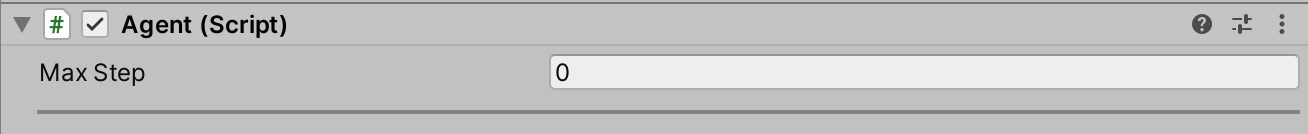
\includegraphics[scale=0.5]{img/agent_komponente}
  \caption{Unity ML-Agents Agenten Komponente}
  \label{fig:agent_komponente}
\end{figure}

Abbildung \ref{fig:agent_komponente} zeigt die Basiskomponente des Agenten. Die Agenten Komponente stellt alle grundlegenden Funktionen des verstärkenden Lernens bereit und implementiert die Verbindung zur Akademie und dem Verhalten des Agenten. Ohne das überschreiben der Funktionen ist die Agentenklasse jedoch ohne Funktion. Die genauen Methoden zur Implementierung eigener Agentenklassen werden näher in Kapitel \ref{subsec:programmierschnittstellen} behandelt. Das einzige Feld zur Konfiguration ist Max Step, welches die maximale Anzahl der Schritte innerhalb einer Episode festlegt.

\begin{figure}[H]
  \centering  
  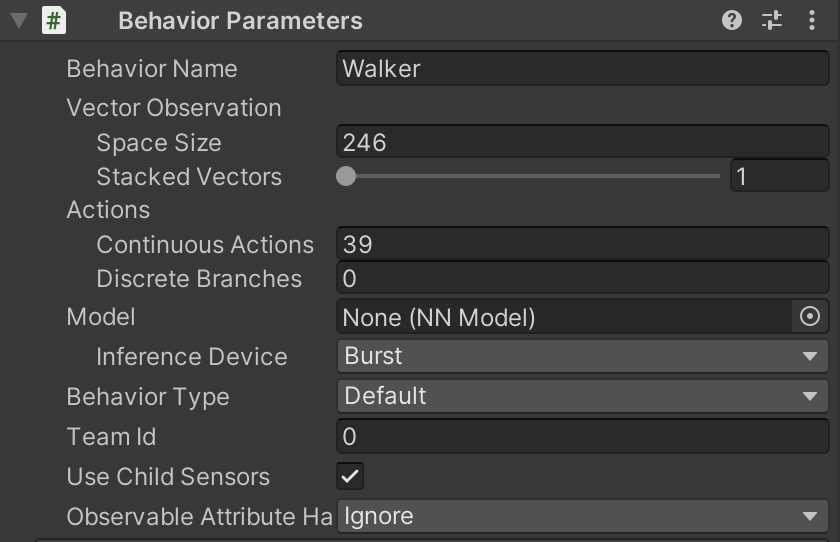
\includegraphics[scale=0.5]{img/verhalten_komponente.png}
  \caption{Unity ML-Agents Verhalten Parameter Komponente}
  \label{fig:verhalten_komponente}
\end{figure}

In Abbildung \ref{fig:entscheidung_anfragen_komponente} ist die Verhaltens Parameter Komponente zusehen. Das Verhalten legt die Ein- und Ausgangsgröße des Modells fest. Für das Training muss ein gleichnamiges Verhalten in der Konfigurationsdatei definiert sein. Um ein bereits trainiertes Verhalten zu verwenden muss im Modell Feld die Modelldatei referenziert werden.

\begin{itemize}
  \item Behaviour Name: Name des Verhaltens / wird in Trainer Konfiguration referenziert
  \item Space Size: Anzahl an Beobachtungen / Inputknoten für NN
  \item Continuous Actions: Anzahl an Aktionen / Outputknoten von NN
  \item Model: Referenz auf bereits trainiertes Modell zur Verwendung in Inferenz
  \item Behaviour Type: Lernmodus Default = Lernen, Heuristic, Inferenz
\end{itemize}

\begin{figure}[H]
  \centering  
  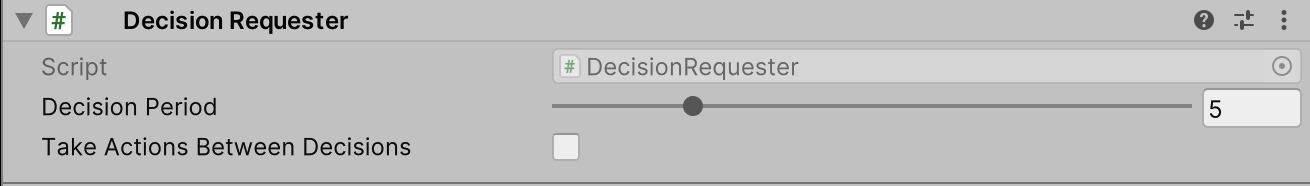
\includegraphics[scale=0.5]{img/entscheidung_anfragen_komponente.png}
  \caption{Unity ML-Agents Entscheidung Anfragen Komponente}
  \label{fig:entscheidung_anfragen_komponente}
\end{figure}

Die Komponente in Abbildung \ref{fig:entscheidung_anfragen_komponente} fragt in regelmäßigen Abständen Entscheidungen an. Das bedeutet es wird eine Beobachtung erstellt. Darauf wird die Beobachtung als Eingangswert für das neuronale Netz genutzt und dann eine Aktion vom neuronalen Netz ausgewählt. Während dem training wird diese Beobachtung zusammen mit der darauf ausgeführten Aktion und der resultierenden Belohnung im Trainingsspeicher abgelegt. Die "Decision Period" gibt an in welchem Interval der Agent eine Entscheidung treffen soll. Das "Kontrollkästchen Take Actions Between Decisions" gibt an ob der Agent die ausgewählte Aktion wiederholen soll bis die nächste Aktion ausgewählt wurde.

\subsection{Programmierschnittstellen}
\label{subsec:programmierschnittstellen}
Die Agenten Komponente enthält einige Funktionen die für das Training eines Agenten implementiert werden müssen. In den folgenden Absätzen werden die Funktionen anhand Beispielen näher erklärt.

\begin{lstlisting}[caption={Agent Funktionen},captionpos=b,label={lst:agent_funktionen}]
public override void CollectObservations(VectorSensor sensor)
{
    sensor.AddObservation(floatObservation);
}

public override void OnActionReceived(ActionBuffers actionBuffers)
{
    var continuousActions = actionBuffers.ContinuousActions;
    movement.x += continuousActions[0]
    movement.y += continuousActions[1]
}

public virtual void FixedUpdate()
{
    AddReward(floatReward);
}
\end{lstlisting}

In der CollectObservations Methoden wird festgelegt welche Daten dem Agent für das Training bereit stehen siehe Listing \ref{lst:agent_funktionen} Zeile 1-3. CollectObservations wird für jede angefragte Entscheidung ausgeführt und das Ergebnis an das NN Modell oder den Python Trainer übergeben.

Wenn eine Entscheidung angefragt wurde und das NN Modell ein Ergebnis liefert wird dieses hier von numerischen Werten in Aktionen umgewandelt. In Listing \ref{lst:agent_funktionen} Zeile 6-11 wird gezeigt wie die Aktion in x und y Bewegung umgesetzt wird.

Im Beispielcode in Listing \ref{lst:agent_funktionen} Zeile 13-16 wird ein Reward in jedem FixedUpdate vergeben über die AddReward Methode die auch Teil der Agenten-Komponente ist. Der Reward kann aber an jeder Stelle im Code vergeben werden, der Code dient hier nur als ein Beispiel.

\begin{lstlisting}[caption={Trainer Konfigurationsdatei},captionpos=b,label={lst:trainer_konfiguration}]
{
behaviors:
  Walker:
    trainer_type: ppo
    hyperparameters:
      batch_size: 2048
      buffer_size: 20480
      learning_rate: 0.0003
      beta: 0.005
      epsilon: 0.2
      lambd: 0.95
      num_epoch: 3
      learning_rate_schedule: linear
    network_settings:
      normalize: true
      hidden_units: 256
      num_layers: 3
      vis_encode_type: simple
    reward_signals:
      extrinsic:
        gamma: 0.995
        strength: 1.0
    keep_checkpoints: 5
    checkpoint_interval: 5000000
    max_steps: 30000000
    time_horizon: 1000
    summary_freq: 30000
environment_parameters:
  environment_count: 100.0
}
\end{lstlisting}

Die Trainings Konfigurationsdatei (siehe Listing \ref{lst:trainer_konfiguration}) enthält mehrere Teile. Der Hyperparameter Teil enthält die Hyperparameter des Maschinellen Lernalgorithmuses (Zeile 5-13), danach folgt der network\_settings Teil welcher die Konfiguration des Neuronalennetzes festlegt (Zeile 14-18). Anschließend folgen noch Konfigurationen für die Belohnungssignale im Bereich reward\_signals (Zeile 19-22) und Einstellungen für die Speicherung der Daten sowie der länge des Trainings (Zeile 23-27). Ganz am Ende der Konfigurationsdatei (Zeile 28-29) befinden sich noch Umgebungsparameter welche erweitert und während dem Training ausgelesen werden können.

